\chapter{Methods and Prototype}

In this section, the used methods are laid out and the implemented prototype is described. 
\section{Methods used}
\subsection{MapReduce}
At the very core of this thesis lies the idea of MapReduce, a programming model made popular by Google and presented in \cite{Dean2008}. Having large data sets to analyse that may not be handled by only few computers, like the millions of Websites gathered by Google each day that have to be indexed fast and reliably, MapReduce  provides a way of automatic parallelisation and distribution of large-scale computations. Users only need to define two types of functions: a map and a reduce function. Each computation expressed by these functions takes a set of input key/value pairs and produces a set of output key/value pairs.
A map function takes an input pair and produces a set of \textit{intermediate} key/value pairs. Once the intermediate values for each intermediate key \textit{I} are grouped together, they are passed to the reduce function. 
The reduce function then takes an intermediate key \textit{I} and the corresponding set of intermediate values (usually supplied as an iterator to the reduce function) and merges them according to user-specified code into a possibly smaller set of values. The resulting key and value are then written to an output file, allowing to handle lists of values that are too large to fit in memory. 

A very simple yet often used MapReduce operation is to count words in a collection of documents, the so called \textit{WordCount}. Below pseudocode demonstrates how one can count all the words in documents using map and reduce functions.

\begin{algorithmic}
\Function{map}{String key, String value}
\State \textit{// key: document name, value: document content}

\For{word $w$ in values}
\State EmitIntermediate($w$, $"1"$);
\EndFor
\EndFunction


\Function{reduce}{String key, Iterator values}
\State \textit{// key: a word, values: a list of "1"'s}
\State int $result$ = 0;
\For{$v$ in values}
\State $result$ += ParseInt($v$);
\EndFor
\State Emit(AsString($result$));
\EndFunction
\end{algorithmic}

The map function splits the received text (\textit{value}) into all corresponding words and for each word, emits its occurrence count (simply a 1). The reduce function then takes, for each word (\textit{key} of the reduce function) individually, these occurrences (\textit{values}) and sums them up, eventually emitting for each word the sum of occurrences (\textit{result}). Although above pseudocode suggests inputs and outputs to be strings, the user specifies the associated types. This means that input keys and values may be of a different domain than the output keys and values (note that the \textit{intermediate} keys and values are from the same domain as the output keys and values). Conceptually, this is expressed as follows:
\newline
\newline
\begin{tabular}{lll}
map	& (k1, v1) & $\to$ list(k2, v2)\\
reduce & (k2, list(v2)) & $\to$ list(v2)
\end{tabular}

The traditional way to view the workflow in a MapReduce program is indicated by Figure \ref{fig:mapreduce_workflow}. A master schedules execution and assigns tasks to workers, which then perform the actual map or reduce on the assigned data. Input data is partitioned into \textit{M} splits with a size of around 16-64 MB per piece to be processed in parallel by different machines, and the intermediate key space is partitioned into \textit{R} pieces, where R usually is the number of available workers for executing reduce but may also be specified by the user. To evenly distribute these pieces, a partitioning function like \textit{hash(key) mod R} may be used. In such a setting, same intermediate keys may not be grouped together, which is done before the reduce action is performed. Additional combination in between may be applied to reduce the amount of data to be distributed among the workers.

\begin{figure}
	\centering	
	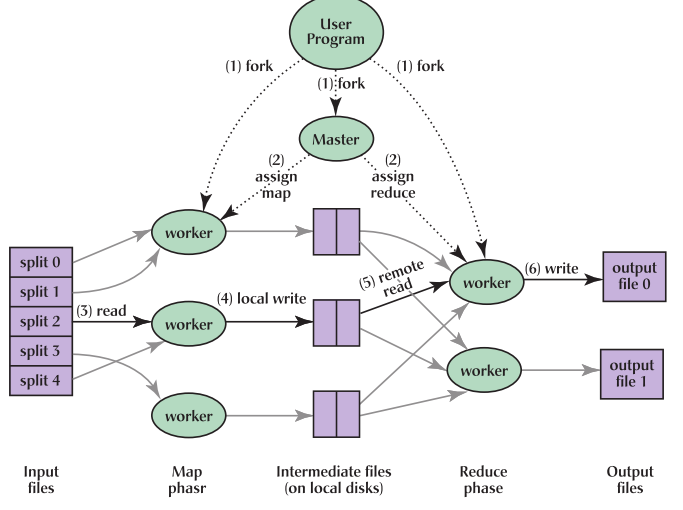
\includegraphics{imgs/mapreduce_workflow}
	\caption{Execution overview in a typical MapReduce program}	
	\label{fig:mapreduce_workflow}
\end{figure} 
\section{Peer-to-Peer Overlay Networks}
\subsection{Definitions and Flavours}
Peer-to-peer (P2P) systems and applications are distributed systems without any centralized control or hierarchical organisation, where the software running at each node is equivalent in functionality \cite{Stoica2001}. Instead of a central server (as present in Client/Server architectures \cite{Schollmeier:2001:DPN:882470.883282}), many hosts (usually referred to as peers) that posses desired contents also handle user requests for them \cite{Chawathe2003}. According to \cite{Schollmeier:2001:DPN:882470.883282}, a P2P network is given if the participants share a part of their own hardware resources (like e.g. processing power or storage capacity), which provide the service and content offered by the network and which are directly accessible by other peers. Peers are, thus, both resource (service  and content) providers and requesters. There exist different flavours of P2P overlay networks but the overall themes may be summarised as "pure" P2P and "hybrid" P2P systems. In a \textit{pure P2P system}, any entity may be removed without the network suffering any service loss. A \textit{hybrid P2P system}, on the other hand, requires a central entity to provide parts of the offered networks. An example of such a hybrid system was Napster \cite{Chawathe2003}. The used P2P system in this work is TomP2P which will be explained shortly.  

\subsection{Discovering Content and Distributed Hash Tables}
The definitions given above demonstrate the need for efficiently discovering content and/or services without using a central server. Central servers may provide O(\textit{1}) lookup of a file's location in the P2P network but also suffers from the problem of being a single point of failure (SPOF), which made Napster very efficient for lookup but also vulnerable for lawsuits \cite{Chawathe2003} and it was certainly not scalable at that time \cite{Ratnasamy:2001:SCN:964723.383072}. However, although being rather resilient to node crashes, without efficient lookup capabilities, P2P networks are \textit{unstructured} and as there is no constraint on where files are placed in the overlay network, queries need to be flooded across the overlay to find the location of the desired content (requiring O(\textit{n}) lookups). Such overlay networks like e.g. Gnutella were, therefore, not scaling. To overcome this, distributed hash tables (DHTs) were introduced, of which the Content-Addressable Network (CAN, \cite{Ratnasamy:2001:SCN:964723.383072}) may be one of the first such design outlines intended to be used in P2P networks. Keys are mapped onto values in a DHT, operations include (among others) typical hash table or hash map operations like put(\textit{key}, \textit{value}), get(\textit{key}): \textit{value}, etc. The idea is that the problem of P2P systems is not the file transfer process which is inherently scalable but finding the peer from whom to retrieve the file\cite{Ratnasamy:2001:SCN:964723.383072}. Thus, the indexing scheme needs to be scalable to make the whole P2P system scalable. Importantly, it requires no centralized control and there is no rigid hierarchical naming structure like e.g. in IP or DNS routing. DHTs make overlay networks \textit{structured} and provide hash-table-like semantics on internet-like scales \cite{Ratnasamy:2001:SCN:964723.383072}. Efficient routing protocols (e.g. Chord\cite{Stoica2001}, Kademlia\cite{Maymounkov:2002:KPI:646334.687801}) reduce lookup complexity to O(log \textit{n}) while lowering node state (the routing entries to other nodes) to O(log \textit{n}) as well. Although there are some limitations to DHTs (e.g. a high churn rate requires O(log \textit{n}) repair operations, keyword searches DHTs by default may only handle exact-match lookups, and many queries may not require an exact recall as they are mostly for well-replicated files and thus, do not justify the overhead of a DHT\cite{Chawathe2003}), they provide a good balance between node state and communication overhead. As TomP2P uses Kademlia as its DHT, its functionality will be briefly outlined next. For more detailed information, please consult the accompanied references.

\subsubsection{title}

\subsubsection{Kademlia}
Kademlia is a P2P DHT with XOR-based metric topology \cite{Maymounkov:2002:KPI:646334.687801}. It combines provable consistency and performance, latency-minimising routing, and a symmetric, unidirectional topology. It minimises number of configuration messages nodes must send to learn about each other, and configuration information spreads automatically as a side-effect of key lookups. Furthermore, nodes have enough knowledge and flexibility to route queries through low-latency paths.
Kademlia contacts only O(log \textit{n}) nodes while searching the system containing \textit{n} nodes. Keys are 160-bit opaque quantities of which each participating computer is assigned one node ID in the 160-bit key space. Key-value pairs are stored on nodes with IDs "close" to the key. Closeness is defined as the bitwise exclusive or (XOR) distance of two nodes' IDs (d(x, y) = x $\mathbin{\oplus}$ y, where x and y are two 160-bit identifiers). A node's ID is a large random number intended to achieve uniqueness. Thus, distance is not used in a geographical sense as "neighbour" nodes may be spread around the world and are only logically considered close in the overlay network due to their small XOR distance. Kademlia treats nodes as leaves in a binary tree, with each node's position determined by the shortest unique prefix of its ID. In a fully-populated binary tree of 160-bit IDs, the magnitude of the distance between two IDs is the hight of the smallest subtree containing them both. If the binary tree is not fully populated, the closest leaf to an ID is the leaf whose ID shares the longest common prefix. For every node, the binary tree is divided into a series of successively lower subtrees that do not contain the node. Every node knows at least one node in each of its subtrees if the subtree contains a node. By successfully querying the known node, contacts are found in lower subtrees until the lookup finally converges to the target node.Thus, any node can locate any other node by its ID.
A Kademlia node stores contact information about each other to route query messages for nodes of distance $2^i$ and $2^{i+1}$ (called \textit{k}-buckets). \textit{k}-buckets are sorted by time last seen (least-recently (head) to most-recently (tail) Appropriate \textit{k}-buckets are updated whenever a Kademlia node receives any message (request or reply) from another node. 


\subsubsection{TomP2P}
The following descriptions are based on \cite{BocekDHT} and \cite{TomP2P}. TomP2P implements, among others, a structured DHT and unstructured broadcasts. These are the main facilities that are used in the present implementation. Additional to the common put(key, value) and get(key): value methods, extended DHT operations that allow storing multiple keys for the same value (add(key, {value}), mimicking Multimap-behaviour) or the same key/value pairs by distinguishing different \textit{domains}. Overall, there are 4 separate keys to distinguish a same value v: location key (the actual k in e.g. put(k, v)), domain key, the content key, and the version key. All domain, content, and version keys are zero if not specified per default. Of these keys, the presented implementation will only make use of location and domain key as these are all that is needed. All keys are of type Number160 in compliance with the aforementioned 160-bit key space of Kademlia, which TomP2P uses for routing. Keys are stored on the nodes with an ID closest to that key. TomP2P makes heavy use of futures to reduce blocking in systems. As each method call will immediately return, the corresponding futures need to implement a listener that specifies what shall happen it is called. Futures may also be cancelled and will, thus, not finish their intended use. Data replication factor is 6 per default.

How to connect peers
How broadcast works
Kademlia routing explained with iterative routing...
References to slides...
\section{Prototype}
\subsection{Discarded Initial Prototypes}
After two failed attempts of implementing a working prototype (see appendix X), it was decided to redesign the prototype from scratch. Initially, a similar design concept as presented in \cite{Steffenel2015} was pursuit, who implemented their MapReduce engine based on the idea that the underlying P2P network should be replaceable and, consequently, the user should not have to care about the actual implementation details. However, during implementation, it became more and more apparent that, to keep the implementation as generic as possible, too many unknowns had to be guessed by the system. Furthermore, over-engineering lead to the fact that the prototype was not possible to test anymore, and problematic assumptions about how to aggregate the data lead to a large number of DHT access calls which slowed down the whole system to an extent that it was not feasible for the execution of MapReduce jobs anymore. Therefore, it was discarded eventually and a new, simpler prototype, which will be presented shortly, was instead implemented. However, due to the pressing time, this last prototype only contained the bare minimum to proof a concept, and has, thus, much improvement and possible redesign to be done. 

\subsection{Final Prototype}
To accommodate the fact that most of the knowledge about the data to process and the intended outcome of a MapReduce job lies with the user, the final prototype gives much more freedom of choice for how the data should be processed. However, this also requires the user to be familiar with the TomP2P framework. The prototype mainly provides a number of helper classes and interfaces to help the user implement a MapReduce job. In the next subsections, these helper classes and interfaces are outlined for users to get a better feeling of how to implement a MapReduce job on their own.

\subsubsection{Rationale}
TODO\newline
What remained from the initial prototypes is the conclusion that, to keep implementation simple and as generic as possible, there needs to be an abstraction for \textit{both} map and reduce functions.

\subsubsection{Task}
\begin{figure}
	\centering	
	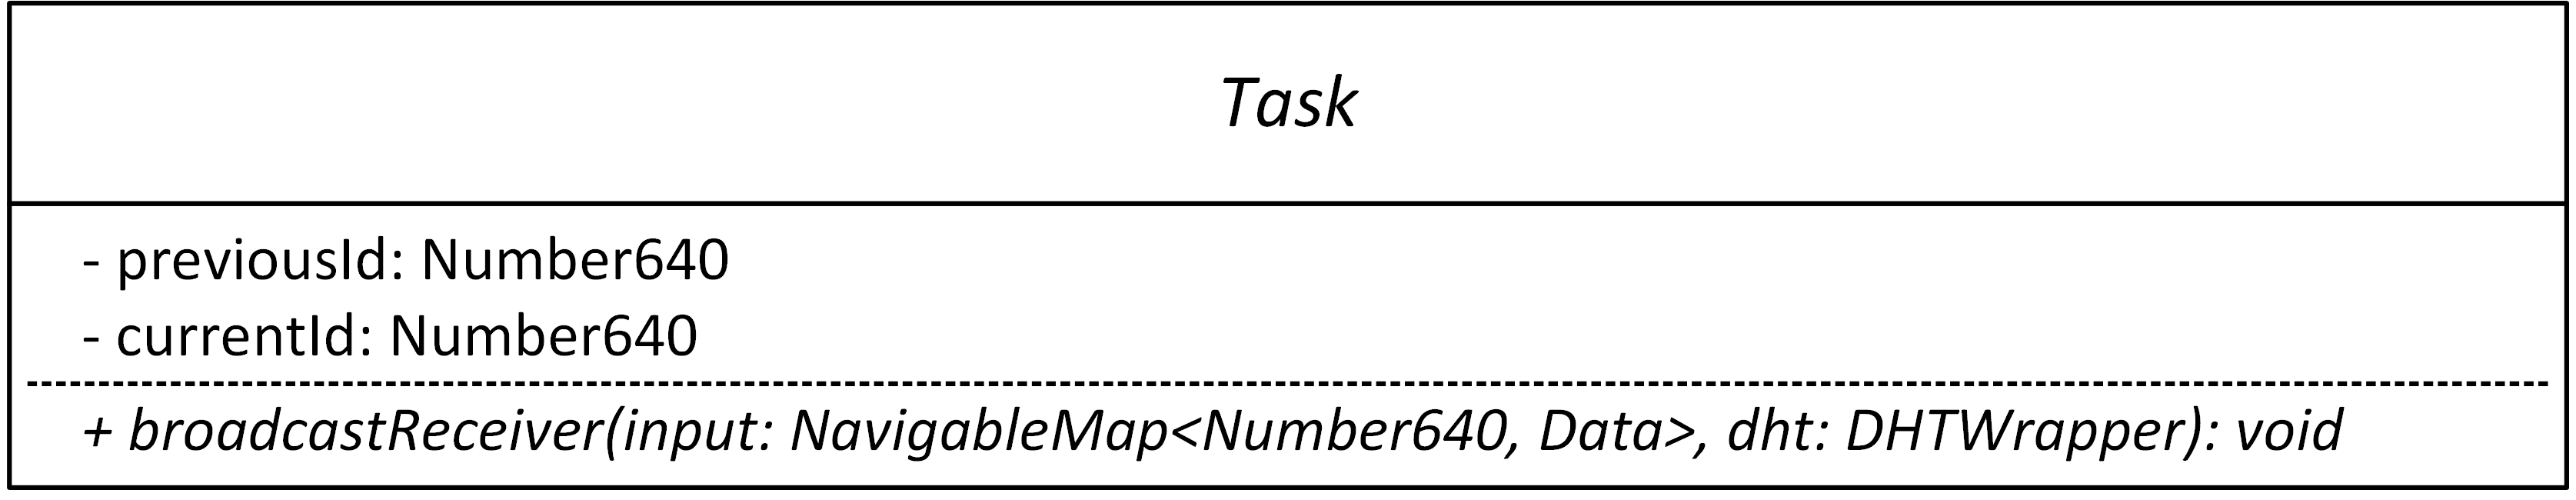
\includegraphics{imgs/taskclass}
	\caption{The Task class - the main extension point for implementing MapReduce jobs}	
	\label{fig:taskclass}
\end{figure}  
The main extension point for a user to implement a MapReduce job is the abstract Task class (Figure \ref{fig:taskclass}). It provides only one method broadcastReceiver(input, dht) for the user to be extended. An extension could be a map or reduce function or any other included procedure to be carried out before or after the actual MapReduce job, like reading, writing, or sorting data items according to a users needs. Thus, Task is the embodiment of the idea of having only one abstraction for all procedures to be carried out during a MapReduce job. Two parameters need to be provided to the broadcastReceiver method: a NavigableMap<Number640, Data> that contains the user-specified data for this Task, and an instance of DHTWrapper. DHTWrapper provides the user with methods to connect and disconnect, put, add, and get data from and to the DHT, and allows for direct emission of broadcasts to all the other nodes. The user-specified data may be anything that this Task needs to execute its job. In the case of a simple WordCount, the initial Task may be to read the data from the user's file system into the DHT. In such a case, this map would contain e.g. the path to the location on the file system, and the Task then would read the data, split it according to the user's specification, and uses the provided DHTWrapper to put the data into the DHT. A last step then is to send a broadcast out, such that other peers connected to the DHT get informed. The broadcast should only be emitted once the task truly finished. Although it is up to the programmer to emit half finished tasks, the reliability increases if the broadcast is only sent when the Task finished completely. If the user, however, knows that the equipment the MapReduce job should run on is reliable enough, Task may be extended to accommodate any performance-increasing measure the user may think of. Thus, the simple interface is actually very powerful for skilled users. Figure \ref{fig:taskclass} also shows that a Task has two Number640 members, previousId and currentId. These two instance variables need to be set by the user to specify which Task comes after which. Especially in the case of the initial Task, the previousId is intended to be null, such that the start of a procedure execution may be determined by the system.
\subsubsection{Job}
To define and start a MapReduce job, there exists one class simply called Job that allows the user to add defined tasks and start the job. Several helper methods like findStartTask or findTask according to the Task's id (see currentId in Figure \ref{fig:taskclass}) are provided as well as the actual start method. The start method takes the same input parameters as the Task's broadcastReceiver method. The intention behind this is that the start method simply looks for the first Task in its Task list (specified by the previousId being null as stated before) and then calls broadcastReceiver with these input parameters on the found first Task. Thus, the first task is a locally executed procedure. In the WordCount example, this task may read the data from the local file system and send it out to the DHT. A broadcast call will then initiate the first non-local procedure, where other peers connected to the DHT may execute the user-specified tasks. Very important are the two method serialize() and deserialize() provided by the Job class. As peers connected on other nodes may not know of the actual Task implementation provided by the user, they need to be serialised and transferred to these nodes. To do so, Job uses the helper class SerializeUtils, which provides two different sets of methods for serialising and deserialising both needed class files and actual instantiated Java objects defined by the user: serializeClassFile/deserializeClassFile turn a class specified by its Class<?> into a byte[] or back to their respective Class<?>, respectively. This allows for the user-defined Task class(es) to be transferred and instantiated on another node across the network without the other node having to know about the .class file(s). The other set of methods provides by SerializeUtils are serializeJavaObject/deserializeJavaObject. While serializeJavaObject turns an instance of the specified class into a byte[], deserializeJavaObject will convert this byte[] back to the object on another node across the network. However, deserializeJavaObject needs the beforehand serialized class files to reliably convert the object back on another node as the class may be unknown when the node receives it at runtime. Thus, SerializeUtils is one of the most important class for allowing the transfer and instantiation of beforehand unknown classes (like user-defined Tasks) on different nodes. Job.serialize() and Job.deserialize() both use two objects to store the serialized data: JobTransferObject and TransferObject. Both classes are simply used for transfer the specified data and contain the byte[] for class files and objects to be instantiated on the node that retrieve the job.
\begin{figure}
	\centering	
	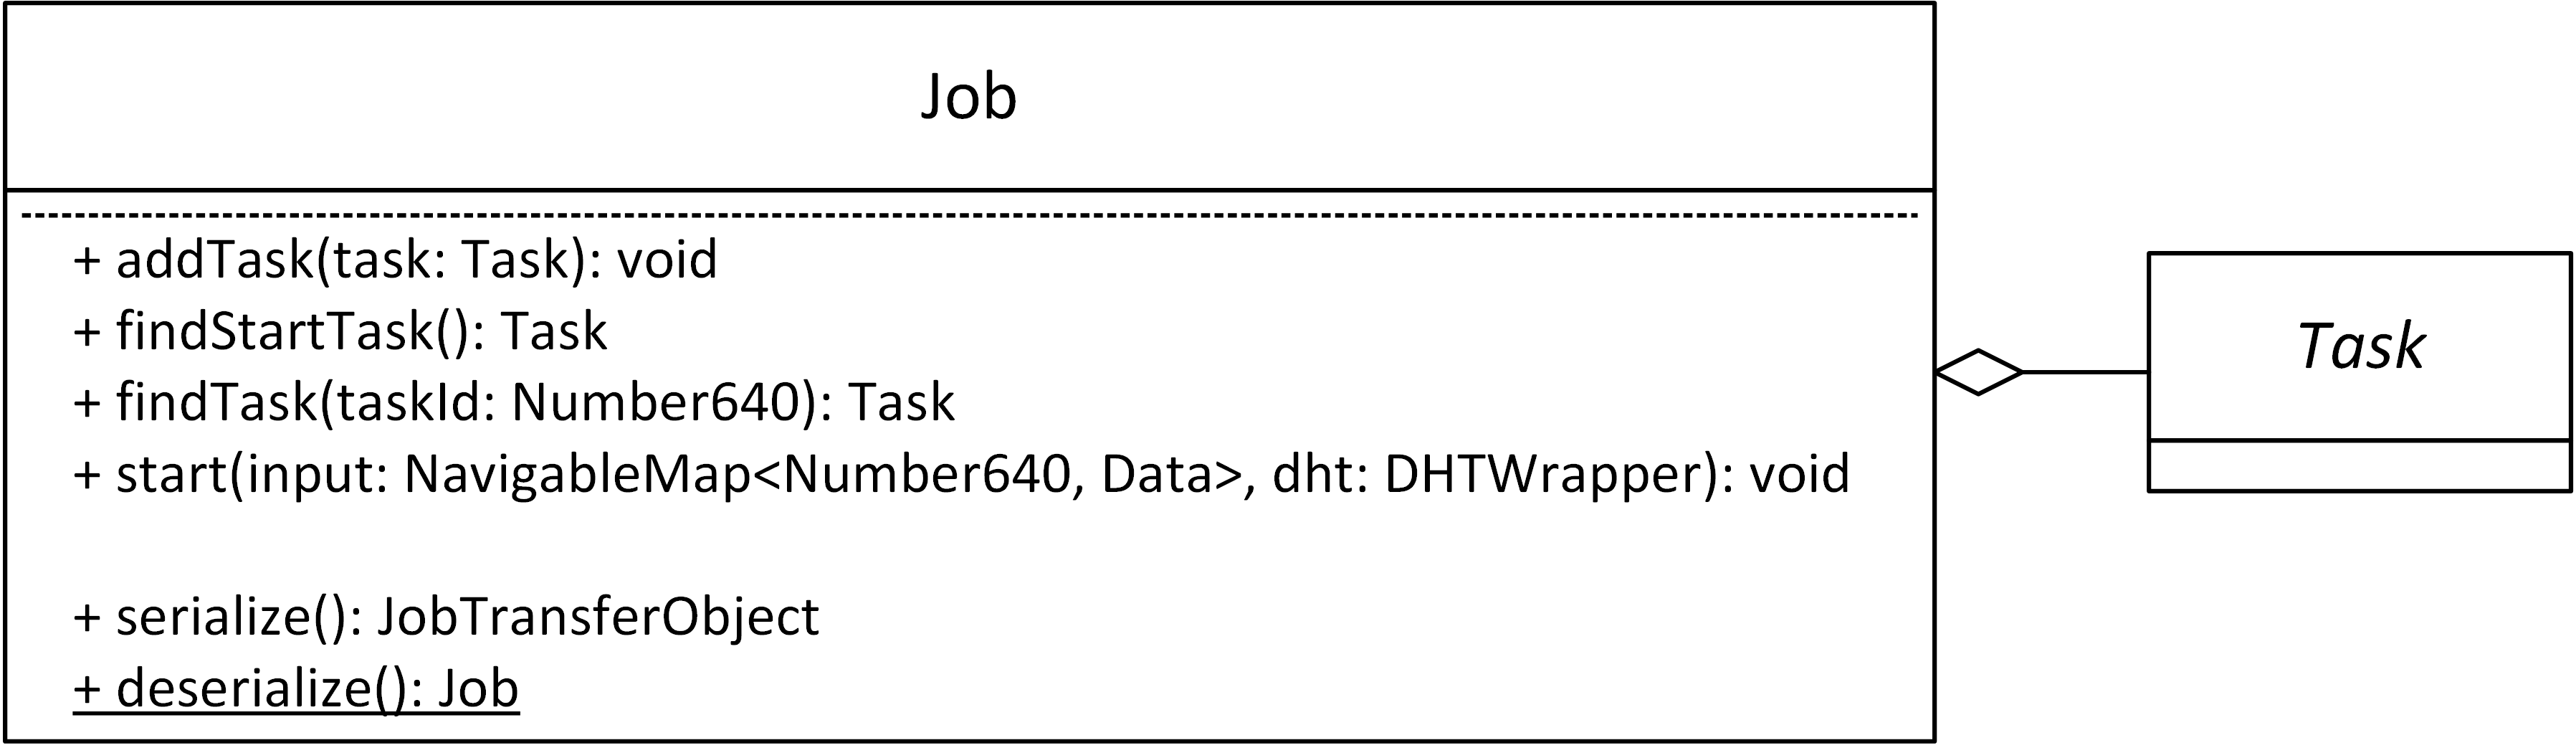
\includegraphics{imgs/jobtask}
	\caption{The Job class - starting point of any MapReduce job}	
	\label{fig:jobtask}
\end{figure} 
\subsubsection{MapReduceBroadcastHandler}
Another important class that has to be used in a MapReduce job is an instantiation of MapReduceBroadcastHandler. Although it is up to the user to define how this broadcast handler is implemented, the execution of a MapReduce job relies on the implementation of its super class' receive(message) method. This method is inherited from StructuredBroadcastHandler and makes sure that all nodes in the network are informed when a new message (e.g. a completed Task) is received. The idea is that, when a new job is submitted to the DHT, the broadcast handler is the instance to retrieve the job and execute the next Task in the MapReduce job for which this message was received. As an example, if the user specified that the map task should emit all words and ones for a file, the broadcast handler will then look for the corresponding next Task to execute (which will count all the ones for that file). Thus, the broadcast handler will, similar to the Job's start method, find the next Task and invoke its broadcastReceiver(input, dht) method. Thus, where Job.start represents the \textit{local} starting point of a MapReduce job, MapReduceBroadcastHandler.receive(message) is the \textit{remote} starting point for all Tasks afterwards.
